% poster.tex
%
% example poster for my Purdue Beamerposter template
%
% Copyright (c) 2017 Dennis Ogbe <dogbe@purdue.edu>
%
% This file is published under the Creative Commons Attribution-NonCommercial
% 4.0 International License. For more information, please visit
% https://creativecommons.org/licenses/by-nc/4.0/

% Sometimes these commands help with Adobe reader
\pdfobjcompresslevel=0
\pdfminorversion=4

\documentclass[pdf]{beamer}

% beamerposter, 36x48 in
\usepackage[orientation=landscape,size=custom,width=121.92,height=91.44, scale=1.8]{beamerposter}

% load required packages. I prefer IEEEtran for equations, but that's a
% personal preference.
\usepackage{IEEEtrantools}

\usepackage{pgf}  % PGF/TikZ is needed for nice plots

\usepackage{caption}
\usepackage{adjustbox}

\usepackage[cmex10]{mathtools} % for math equations
\usepackage{amssymb}
\usepackage{bm}

\usepackage{framed}

\usefonttheme[onlymath]{serif}
\usepackage{mathrsfs}
\usepackage[utf8]{inputenc}
\usepackage{printlen}

% bibliography
\usepackage[bibstyle=ieee,citestyle=numeric,backend=biber]{biblatex}
\addbibresource{all.bib}
% if the following were not set, biblatex would try to insert a section on
% every frame, which breaks beamer
\defbibheading{bibliography}[\bibname]{}
% modify the font size of the \cite commands
% we want numbers instead of symbols in the bibliography
\setbeamertemplate{bibliography item}[text]
% make it small
\renewcommand*{\bibfont}{\scriptsize}

% useful to set this when using Inkscape SVG figures
\graphicspath{{./figures/}}
\usetheme{purduegoldposter}

% some extra colors
\definecolor{Red}{HTML}{FF0000}
\definecolor{Green}{HTML}{085C11}
\definecolor{Blue}{HTML}{2D2D9F}

% clear out the footer
\setbeamertemplate{footline}{}

\usepackage{lmodern}

% underline hacking
\usepackage{soul}


\newcommand{\phone}{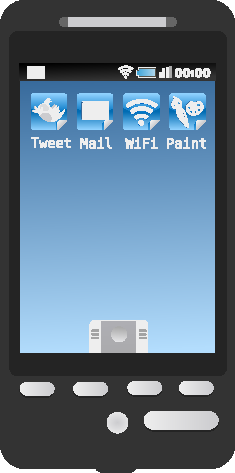
\includegraphics[width=0.22cm]{./figures/1281043443.pdf}}
\newcommand{\basestation}{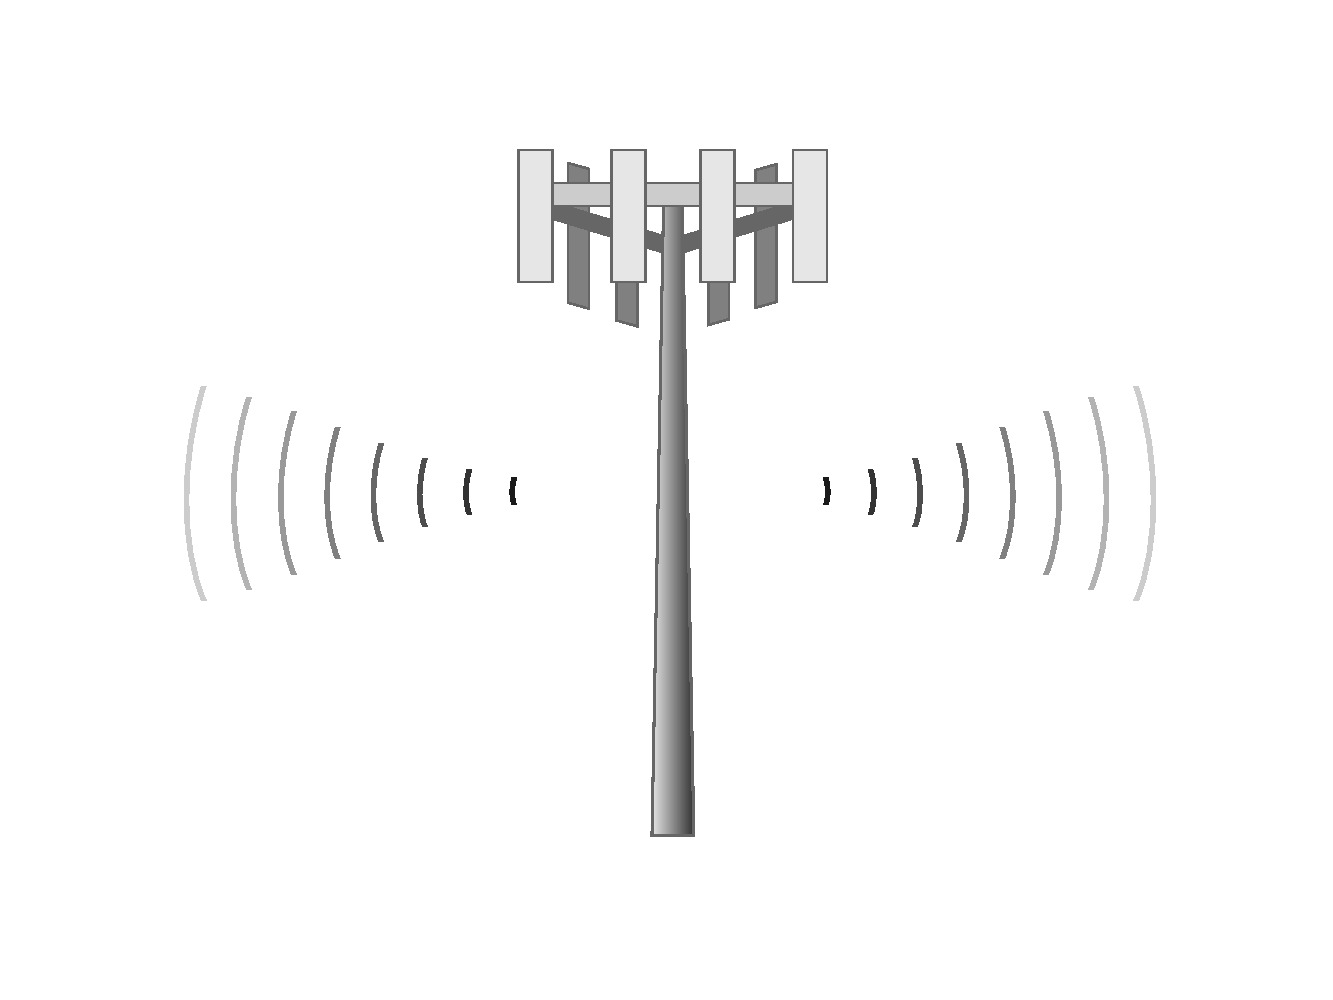
\includegraphics[width=3cm]{./figures/CellTower.pdf}}
\newcommand{\smallcell}{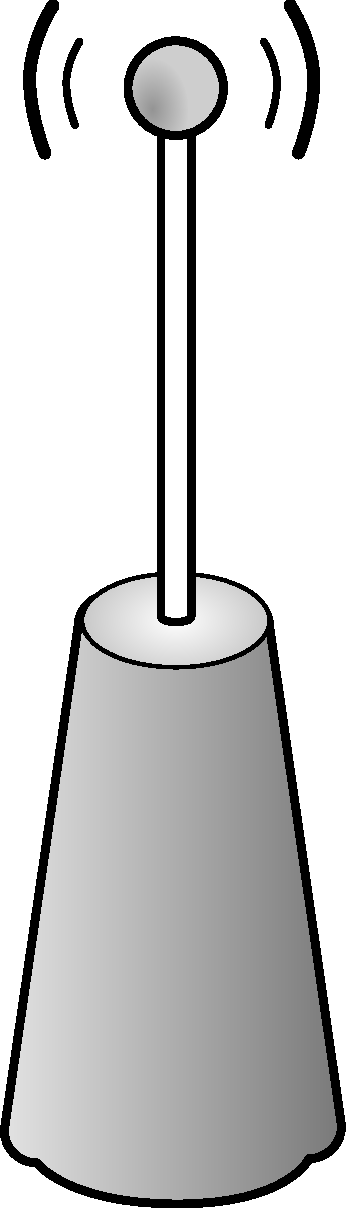
\includegraphics[width=0.25cm]{./figures/Anonymous-Wireless-Transmitter.pdf}}

\newcommand{\smallcellnw}{%
  \begin{tikzpicture}[
    x=1cm, y=1cm,
    shorten < = 0.3cm,
    shorten > = 0.3cm
    ]
    % base station
    \node at (0,0) {\basestation};
    \draw[thick, color=blue!30] (0,0) ellipse (4.5 and 2.5);

    % left small cell
    \node at (-2.7, -0.2) {\smallcell};
    \draw[thick, color=black!60] (-2.7, -0.2) ellipse(1.2 and 1);
    \draw[shorten < = 0.5cm, ultra thick, dashed, color=red!60] (0, 0.8) -- (-2.7, 0.1);
    \node at (-3.5, -0.2) {\phone};
    \node at (-1.9, -0.2) {\phone};
    \node at (-3.3, 0.35) {\phone};
    \node at (-3, -0.8) {\phone};

    % right bottom small cell
    \node at (1.7, -1.2) {\smallcell};
    \draw[thick, color=black!60] (1.7, -1.2) ellipse(1.2 and 1);
    \draw[shorten < = 0.6cm, ultra thick, dashed, color=red!60] (0, 0.8) -- (1.7, -0.9);
    \node at (2.5, -1) {\phone};
    \node at (1, -0.8) {\phone};
    \node at (2.1, -1.8) {\phone};
    \draw[shorten > = 0.1cm, shorten < = 0.2cm, very thick, dashed, color=red] (2.5, -1) -- (1.7, -0.9);

    % right top small cell
    \node at (2.1, 1.1) {\smallcell};
    \draw[thick, color=black!60] (2.1, 1.1) ellipse(1.2 and 1);
    \draw[shorten < = 0.4cm, ultra thick, dashed, color=red!60] (0, 0.8) -- (2.1, 1.5);
    \node at (2.7, 1.1) {\phone};
    \node at (1.5, 1.6) {\phone};

    % extra phones
    \node at (-1.5, 1.8) {\phone};
    \node at (-1, 1) {\phone};
    \node at (-0.5, -1.5) {\phone};
    \node at (-1, -1.7) {\phone};
  \end{tikzpicture}
}

\newcommand{\dfpipelining}{%
  \begin{tikzpicture}[
    x = 1.2cm,
    y = 1.2cm,
    ]
    % first block
    \draw (0,3) rectangle (9,4);
    \foreach \x in {1, 2, 3, 4, 5, 6, 7, 8}
    \draw (\x, 3) -- (\x, 4);
    % second block
    \draw (9, 0) rectangle (18, 1);
    \foreach \x in {10, 11, 12, 13, 14, 15, 16, 17}
    \draw (\x, 0) -- (\x, 1);
    % ghost blocks
    \begin{scope}[shift={(0.4, 0)}, dashed, color=gray!90]
      \draw (9, 3) rectangle (18, 4);
      \foreach \x in {10, 11, 12, 13, 14, 15, 16, 17}
      \draw (\x, 3) -- (\x, 4);
      \draw  (22, 0) -- (18, 0) -- (18, 1) -- (22, 1);
      \foreach \x in {19, 20, 21}
      \draw (\x, 0) -- (\x, 1);
      \draw (9, 3) -- (18, 1);
      \draw (18, 3) -- (22, 2);
      \draw[->, shorten > = 3pt, ultra thick]
      (9, 5.5) -- (9, 4) node[midway, right] {\small Start encode};
    \end{scope}
    % diag lines
    \begin{scope}[color=blue!90]
      \draw (0, 3) -- (9, 1);
      \draw (9, 3) -- (18, 1);
    \end{scope}
    % vert lines
    \foreach \x in {0, 9, 18}
    \draw[dashed](\x, -1) -- (\x, 4.5);
    % arrows
    \draw[<->, shorten < = 1pt, shorten > = 1pt]
    (0, -0.7) -- (9, -0.7) node[midway, below] {\small $T_{1}$};
    \draw[<->, shorten < = 1pt, shorten > = 1pt]
    (9, -0.7) -- (18,  -0.7) node[midway, below] {\small $T_{2}$};
    % annotations
    \draw[->, shorten > = 3pt, ultra thick, color=black!50!green]
    (0, 5.5) -- (0, 4) node[midway, right] {\small Start encode};
    \draw[->, shorten < = 3pt, ultra thick, color=black!10!orange]
    (18,  -1) -- (18, -2.5) node[midway, right] {\small Extract msg};
    \node[anchor=east, shift={(-0.2, 0.5)}] at (0, 3) {\small Source Tx};
    \node[anchor=east, shift={(-0.2, 0.5)}] at (0, 0) {\small Relay Tx};
  \end{tikzpicture}
}%

\newcommand{\afpipelining}{
    \begin{tikzpicture}[
    x = 1.2cm,
    y = 1.2cm,
    ]
    % first block
    \draw (0,3) rectangle (9,4);
    \foreach \x in {1, 2, 3, 4, 5, 6, 7, 8}
    \draw (\x, 3) -- (\x, 4);
    % second block
    \draw (1, 0) rectangle (10, 1);
    \foreach \x in {2, 3, 4, 5, 6, 7, 8, 9}
    \draw (\x, 0) -- (\x, 1);
    % ghost blocks
    \begin{scope}[shift={(0.4, 0)}, dashed, color=gray!90]
      \draw (14.5, 3) -- (9, 3) -- (9, 4) -- (14.5, 4);
      \foreach \x in {10, 11, 12, 13, 14}
      \draw (\x, 3) -- (\x, 4);
      \draw (14.5, 0) -- (10, 0) -- (10, 1) -- (14.5, 1);
      \foreach \x in {11, 12, 13, 14}
      \draw (\x, 0) -- (\x, 1);
      \foreach \x in {9, 10, 11, 12, 13}
      \draw (\x, 3) -- (\x+1, 1);
      \draw (14, 3) -- (14.5, 2);
      \draw[->, shorten > = 3pt, ultra thick]
      (9, 5.5) -- (9, 4) node[midway, right] {\small Start encode};
    \end{scope}
    % diag lines
    \begin{scope}[color=blue!90]
      \foreach \x in {0, 1, 2, 3, 4, 5, 6, 7, 8, 9}
      \draw (\x, 3) -- (\x+1, 1);
    \end{scope}
    % vert lines
    \foreach \x in {0, 9, 10}
    \draw[dashed](\x, -1) -- (\x, 4.5);
    % arrows
    \draw[<->, shorten < = 1pt, shorten > = 1pt]
    (0, -0.7) -- (9, -0.7) node[midway, below] {\small $T_{1}$};
    \draw[<->, shorten < = 1pt, shorten > = 1pt]
    (9, -0.7) -- (10,  -0.7) node[midway, below] {\small $1$};
    % annotations
    \draw[->, shorten > = 3pt, ultra thick, color=black!50!green]
    (0, 5.5) -- (0, 4) node[midway, right] {\small Start encode};
    \draw[->, shorten < = 3pt, ultra thick, color=black!10!orange]
    (10,  -1) -- (10, -2.5) node[midway, right] {\small Extract msg};
    \node[anchor=east, shift={(-0.2, 0.5)}] at (0, 3) {\small Source Tx};
    \node[anchor=east, shift={(-0.2, 0.5)}] at (0, 0) {\small Relay Tx};
  \end{tikzpicture}
}

\newcommand{\tcpipelining}{%
  \begin{tikzpicture}[
    x = 1.2cm,
    y = 1.2cm,
    ]
    % first block
    \draw (0,3) rectangle (9,4);
    \foreach \x in {1, 2, 3, 4, 5, 6, 7, 8}
    \draw (\x, 3) -- (\x, 4);
    % second block
    \draw (3, 0) rectangle (12, 1);
    \foreach \x in {4, 5, 6, 7, 8, 9, 10, 11}
    \draw (\x, 0) -- (\x, 1);
    % ghost blocks
    \begin{scope}[shift={(0.4, 0)}, dashed, color=gray!90]
      \draw (15.5, 3) -- (9, 3) -- (9, 4) -- (15.5, 4);
      \foreach \x in {10, 11, 12, 13, 14, 15}
      \draw (\x, 3) -- (\x, 4);
      \draw (15.5, 0) -- (12, 0) -- (12, 1) -- (15.5, 1);
      \foreach \x in {13, 14, 15}
      \draw (\x, 0) -- (\x, 1);
      \draw (9, 3) -- (12, 1);
      \draw (12, 3) -- (15, 1);
      \draw (15, 3) -- (15.5, 2.5);
      \draw[->, shorten > = 3pt, ultra thick]
      (9, 5.5) -- (9, 4) node[midway, right] {\small Start encode};
    \end{scope}
    \begin{scope}[color=blue!90]
      \foreach \x in {0, 3, 6, 9}
      \draw (\x, 3) -- (\x+3, 1);
    \end{scope}
    % vert lines
    \foreach \x in {0, 9, 12}
    \draw[dashed](\x, -1) -- (\x, 4.5);
    % arrows
    \draw[<->, shorten < = 1pt, shorten > = 1pt]
    (0, -0.7) -- (9, -0.7) node[midway, below] {\small $T_{1}$};
    \draw[<->, shorten < = 1pt, shorten > = 1pt]
    (9, -0.7) -- (12,  -0.7) node[midway, below] {\small $\Delta$};
    % annotations
    \draw[->, shorten > = 3pt, ultra thick, color=black!50!green]
    (0, 5.5) -- (0, 4) node[midway, right] {\small Start encode};
    \draw[->, shorten < = 3pt, ultra thick, color=black!10!orange]
    (12,  -1) -- (12, -2.5) node[midway, right] {\small Extract msg};
    \node[anchor=east, shift={(-0.2, 0.5)}] at (0, 3) {\small Source Tx};
    \node[anchor=east, shift={(-0.2, 0.5)}] at (0, 0) {\small Relay Tx};
  \end{tikzpicture}
}%


\newcommand{\sthr}{%
  \begin{tikzpicture}[
    x=1.8in, y=1.8in,
    shorten <=0.8in,
    shorten >=0.8in,
    ]
    \draw[thick] (-3, 0) circle (0.4) node {$S$};
    \draw[thick] (0, 0) circle (0.4) node {$R$};
    \draw[thick] (3, 0) circle (0.4) node {$D$};
    \draw[-{Latex[width=0.8cm, length=1.1cm]},ultra thick] (-3, 0) -- (0, 0);
    \draw[-{Latex[width=0.8cm, length=1.1cm]},ultra thick] (0,0) -- (3, 0);

    \node at (-3, 0.66) {$X(t)$};
    \node at (0, 0.66) {$Y(t)$\hspace{1.5in} $V(t)$};
    \node at (3, 0.66) {$Z(t)$};
  \end{tikzpicture}
}


% set title and author
\title{Transcoding: A New Strategy for Relay Channels}
\author{Dennis Ogbe, Chih-Chun Wang, David J. Love}

\begin{document}
%\setuldepth{\textbf{Theory}}

\begin{frame}[t]
% title
\begin{textblock}{1}(0,0)
  \begin{tcolorbox}[
    % colors
    colback=MoonDustGray,
    colframe=black,
    % rule widths & arcs
    toprule=0pt,
    leftrule=0pt,
    rightrule=0pt,
    bottomrule=0.3in,
    arc=0pt,
    % padding
    sidebyside,
    lower separated=false,
    righthand width=0.3\paperwidth,
    boxsep=0.25in,
    % text & logo alignment
    halign upper=left,
    halign lower=right
    ]
    \huge{\textbf{\inserttitle}}

    \Large{\emph{\insertauthor}}

    \normalsize{Purdue University, School of Electrical and Computer Engineering, West Lafayette, IN 47907, USA}

    \tcblower
    \hfill
    \raisebox{0.4in}{
\includegraphics[width=7.5in]{./logos/Purdue-Sig-Black-cmyk.pdf}}
    \hfill
    
\includegraphics[width=3in]{./logos/NSF_4-Color_bitmap_Logo.png}
    \hfill
   \raisebox{0.2in}{
\includegraphics[width=3in]{./logos/CSoI-logo-print.png}}
\end{tcolorbox}
\end{textblock}
% column 1
\begin{textblock}{0.33}(0.005,0.12)
  \begin{center}
    \ul{\textbf{Rise of Multi-hop, Low-latency Communication}}
  \end{center}
  \begin{itemize}
  \item Number of wireless devices continues to grow
  \item Many ``new'' devices will be low-power Internet of Things (IoT) devices
  \item Potentially \textbf{no direct connection to base station}
  \item Cellular: Move to \textbf{small cell networks}, in-band wireless (self-)backhauling
  \end{itemize}
  \begin{center}
    \resizebox{0.9\textwidth}{!}{\smallcellnw}

  \small{Small cell network with wireless backhaul}
\end{center}
\begin{itemize}
\item Additionally: Growing focus on \textbf{low latency}
\item Sub-1ms latency in IMT-2020
\end{itemize}

\hrulefill

\begin{center}
  \ul{\textbf{The Relay Channel:}}\\
      \ul{\textbf{A Classic Problem in Information Theory}}
\end{center}
\begin{itemize}
\item Lots of focus from industry \& academia since 1970s
\end{itemize}
\begin{center}
  \fbox{\resizebox{0.65\textwidth}{!}{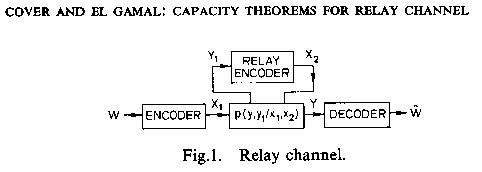
\includegraphics{./figures/cover-relay.pdf}}}
\end{center}
\begin{itemize}
\item Many different design philosophies: Compress-\&-Forward~\cite{cover-elgamal-relay}, Hash-\&-Forward~\cite{cover-kim-deterministic}, Compute-\&-Forward~\cite{nazer-compute-f}, Noisy Network Coding~\cite{lim-nnc}
\item De-facto industry standard: Decode-\&-Forward (DF)~\cite{cover-elgamal-relay}
\item \textbf{Traditional schemes focus on capacity rather than delay performance} ($\Rightarrow$ long block lengths)
\item Our interest: Low latency, short, \textbf{finite block lengths}
\item Amplify-\&-Forward (AF) gives best delay performance but suffers throughput loss due to noise build-up
\end{itemize}
\end{textblock}

% column 2
\begin{textblock}{0.33}(0.335,0.12)
  \begin{center}
    \ul{\textbf{Separated Two-hop Relay Channel}}

    \vspace{1cm}\sthr
  \end{center}
  \begin{itemize}
  \item No connection between source and destination
  \item ``Degraded'' relay channel, DF achieves capacity (with infinite delay)
  \end{itemize}
  \begin{center}
    \ul{\emph{Decode-\&-Forward}}
  \end{center}
  \begin{itemize}
  \item Error control through \textbf{coding at source and relay}
  \item End-to-end delay: $T = T_{1} + T_{2}$
  \item Pipelined coding rate:
    \[\displaystyle R_{DF}(T,\epsilon) = \frac{\log M}{\mathrm{max}\left(T_{1}, T_{2}\right)}\]
  \end{itemize}
  \begin{center}
    \dfpipelining
  \end{center}
  \begin{center}
    \ul{\emph{Amplify-\&-Forward}}
  \end{center}
  \begin{itemize}
  \item No error correction at relay $\Rightarrow$ \textbf{noise accumulation}
  \item End-to-end delay: $T = T_{1} + 1$
  \item Pipelined coding rate:
    \[\displaystyle R_{AF}(T,\epsilon) = \frac{\log M}{T_{1}}\]
  \end{itemize}
  \begin{center}
    \afpipelining
  \end{center}

  {\color{Red} \textbf{Transcoding as ``middle ground'' between AF and DF}
    \begin{itemize}
    \item\color{Red} Can be viewed as ``smart'' AF with error protection
    \item\color{Red} Improved coding rate in low latency regime
    \end{itemize}}
\end{textblock}

% column 3
\begin{textblock}{0.33}(0.665,0.12)
  \begin{center}
    \ul{\textbf{Transcoding}}
  \end{center}
  \begin{itemize}
  \item Idea: Relay processes sub-blocks of size $\Delta$
  \item Structure in sub-blocks $\Rightarrow$ \textbf{Error control at relay}
  \item End-to-end delay: $T = T_{1} + \Delta$
  \item Pipelined coding rate:
    \[\displaystyle R_{TC}(T,\epsilon) = \frac{\log M}{T_{1}}\]
  \end{itemize}
  \begin{center}
    \tcpipelining
  \end{center}
  \begin{center}
    \ul{\emph{Example: $\Delta = 8$}}~\cite{wang-transcoding-allerton}
  \end{center}
  \begin{itemize}
  \item Binary symmetric channel on both hops
  \item Take sub-blocks from (8,4) extended Hamming Code
  \item Parameters: $p_{1} = 0.04$, $p_{2} = 0.13$, $\epsilon = 10^{-3}$
  \item Normal approximation~\cite{polyanskiy} to evaluate rate-delay tradeoff
  \end{itemize}\vspace*{0.7cm}
  \begin{center}
    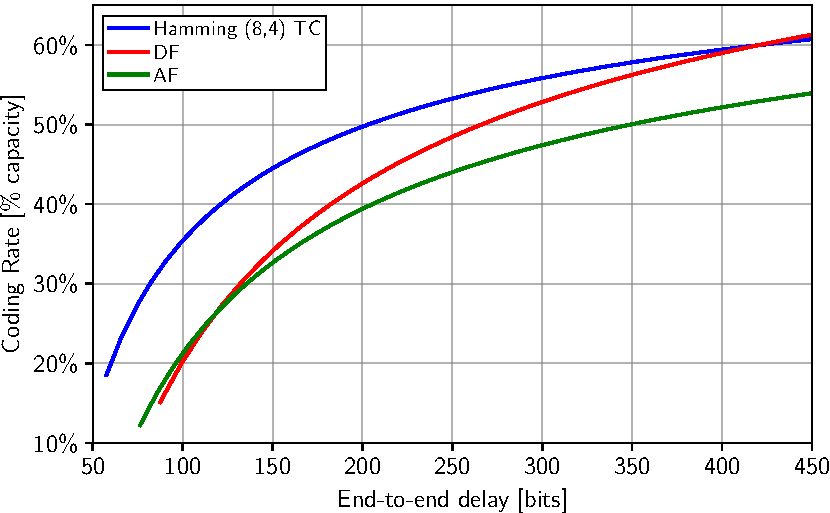
\includegraphics[width=0.85\textwidth]{./plots/plot.pdf}
  \end{center}\vspace{-20pt}
  \hrulefill

  \begin{center}
    \ul{\textbf{Ongoing Work}}
  \end{center}
  \begin{itemize}
  \item Random code construction \& analysis
  \item General transcoder design theory
  \item Extension to multi-hop \& fading channels
  \end{itemize}
\end{textblock}

% bilbliography
\begin{textblock}{0.66}(0.335,0.89)
  \hrulefill

  \printbibliography
  \scriptsize This material is based upon work supported in part by the National Science Foundation under Grant No. CNS-1642982.
\end{textblock}

\end{frame}
\end{document}

%%% Local Variables:
%%% mode: latex
%%% TeX-master: t
%%% End:
